\chapter{Analysis and Discussion}
\label{analysis}

\section{Patterns}
\subsection{Detection}
There are more than 100,000 times more similar sequences found in the
scale/filter coefficients than in the wavelet/shift coefficients. The large
difference in number of sequences found between the two types of coefficients
is due to the fact that the LOC metric is a cumulative metric. The typical
trend of a LOC signal is growth. This makes finding similar sequences using
shift coefficients (i.e., along the time axis) less likely.

\paragraph{}
No patterns were detected in shift coefficients. This can be explained by the
fact that the 16 similar sequences in shift coefficients are not similar within
the same group of sequences.

Additionally, the shift coefficients are incomparable to the filter coefficients
because they were found in a fundamentally different way of signal
transformation. Mixing both types of coefficients would neglect the way the
coefficients were found and invalidate the patterns comprising sequences of
both types of coefficients.

\subsection{Similarity}
The patterns that were detected show strong similarity among signals. The
similarity was demonstrated in Figure \ref{figure:patterns_plots} in section
\ref{section:seqs_patterns}. The figure presents an arbitrary pattern and its
occurrences across different projects. The figure also demonstrates how wavelet
transforms 'smooths out' differences in details by scaling and filtering the
signals.

\paragraph{}
One of the properties of the Haar function is that it is reversible. This
means that it is possible to pick any wavelet on any level of decomposition
that resulted from Haar transform and use it to re-compose the original signal.
This is a useful property for testing a pattern. Figure
\ref{figure:type_a_pattern} shows the type A pattern \#3256 projected onto the
original signals of two projects.

\begin{figure}[H]
\caption{Type A pattern \#3256 in two projects}\label{figure:type_a_pattern}
\centering
	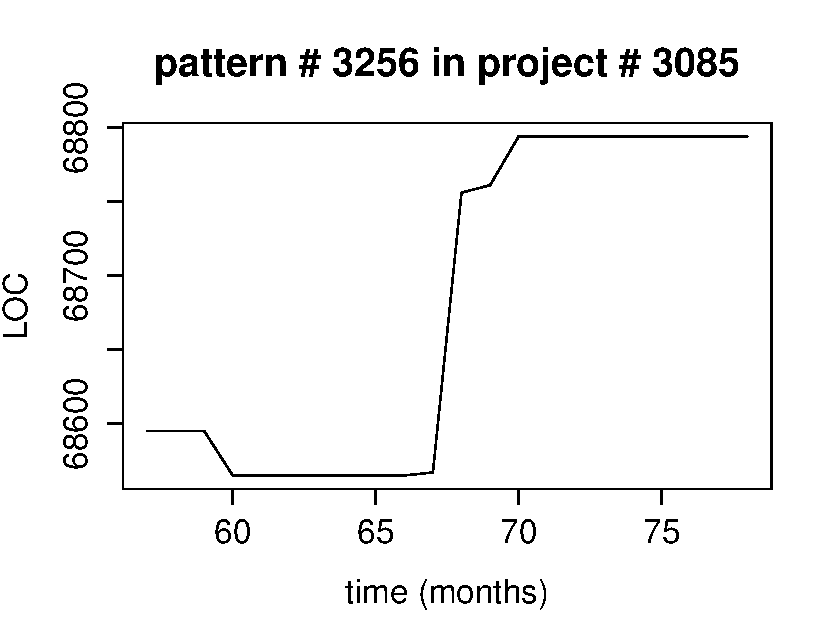
\includegraphics[width=196pt]{images/pattern_a_3085.pdf}
	\hspace{1em}
	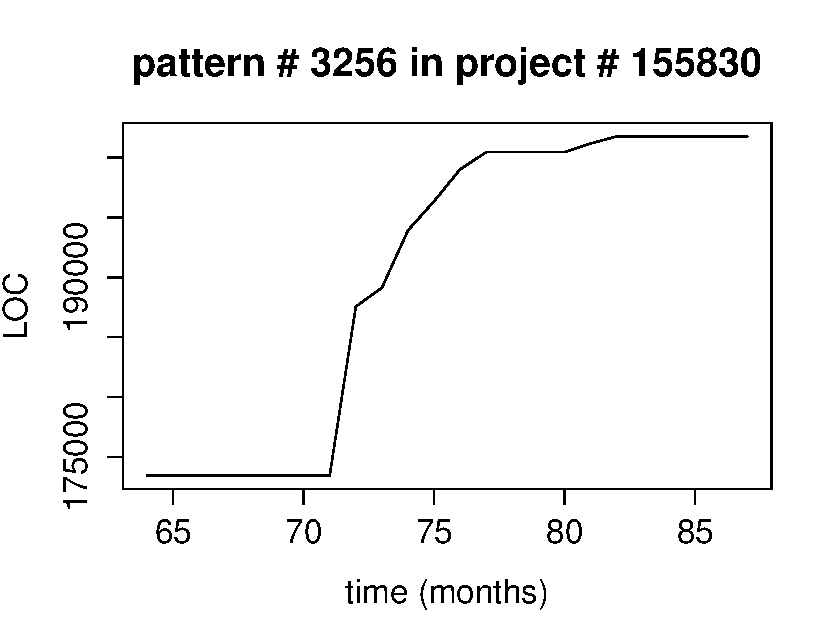
\includegraphics[width=196pt]{images/pattern_a_155830.pdf}
\end{figure}

\indent
Figure \ref{figure:type_a_pattern} shows the wavelets of the occurrence of type
A pattern \#3256 in two dead projects. The pattern starts near, and lasts until
the end of code evolution of the projects. This figure shows that the pattern
ends in a stagnation of LOC change. The shapes of both wavelets are similar,
even though the wavelets are not scaled in this figure -- project \#3085 is
about 30\% smaller than project \#155830 when comparing the LOC values.\\

\noindent
Manual evaluation using the commit logs of these two projects revealed that:

\begin{itemize}
	\item The rise in LOC in the signal of project \#3085 started in its
		67\textsuperscript{th} month of age. It is caused by an update to a file
		with an addition of about 200 lines of code. This does not seem much, but
		relative to the project it is significant and sufficient to shape the
		pattern.

	\item The rise in LOC in the signal of project \#155830 starting in its
		72\textsuperscript{nd} month appears to be caused by a fix of a broken build
		and happened after 25 months of no LOC changes. As far as can be told from
		the commit logs, many lines of code (approximately 10,000) had to be added in
		order to fix the build.
\end{itemize}

\noindent
The flat line starting at month 70 in project \#3085 and at month 83 in project
\#155380 indicate a stagnation in LOC changes and lasts for 15 and 12 months
respectively.

\subsection{Warning signs}
The classification of the patterns detected in dead projects (see section
\ref{section:patterns_dead}) was needed to distinguish possible warning signs
from other recurring events. The type A patterns were expected to be the best
candidates for representing warning signs because of the property that they
last until the end of code evolution of a dead project.

\paragraph{}
Type B patterns are the patterns not lasting until the end of code evolution of
dead projects. The typical shape of the type B patterns found in LOC signals in
this study are sub-linear growth in LOC. The other two common shapes of type B
patterns is an almost super-linear growth sine shape and super-linear decay.
The latter shows a free fall in LOC. Figure \ref{figure:type_b_pattern}
illustrates all three shapes.

\begin{figure}[H]
\caption{Typical type B patterns}\label{figure:type_b_pattern}
\caption*{\footnotesize\textit{\\[1em](left) Sub-linear growth\\(center)
Super-linear/sine-shaped growth\\(right) Super-linear decay}\\[1em]}
\centering
	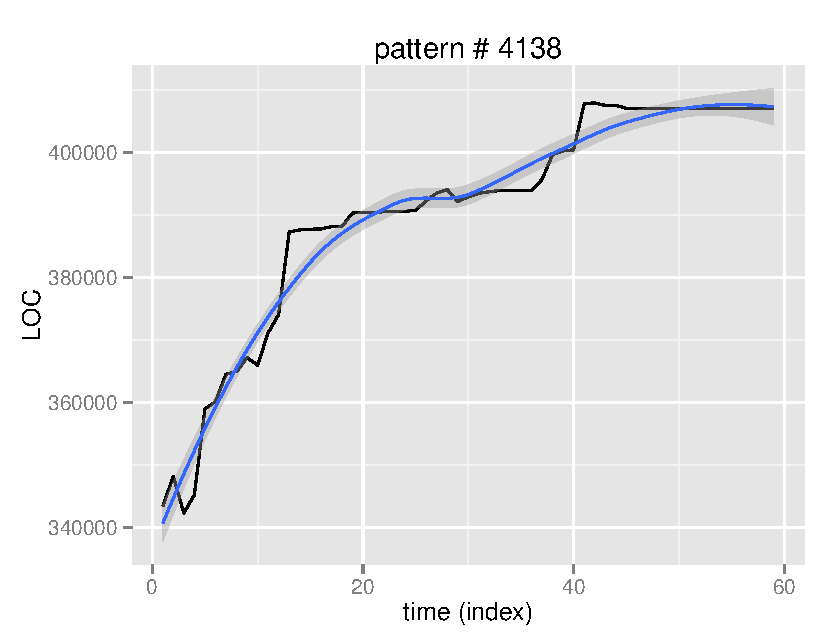
\includegraphics[width=128pt]{images/pattern_b_sub.pdf}
	\hspace{1em}
	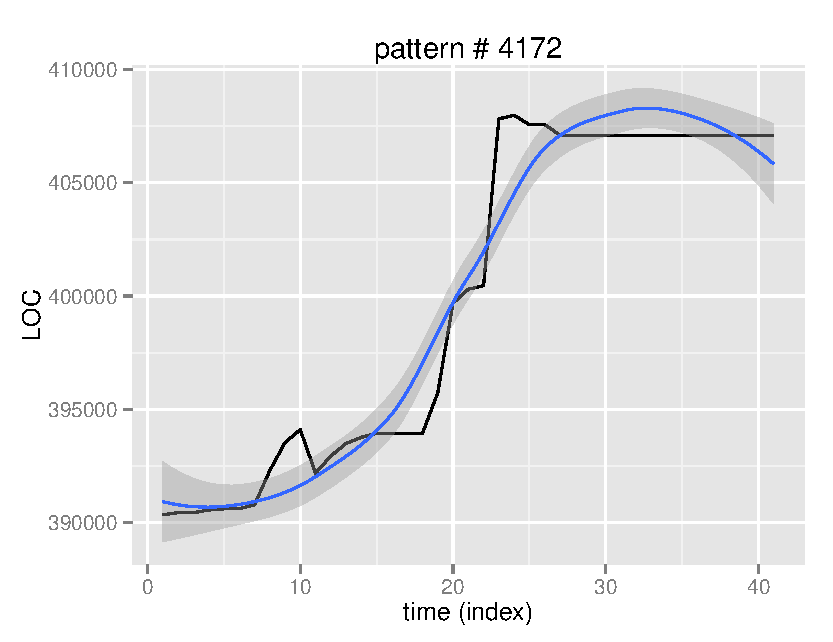
\includegraphics[width=128pt]{images/pattern_b_sine.pdf}
	\hspace{1em}
	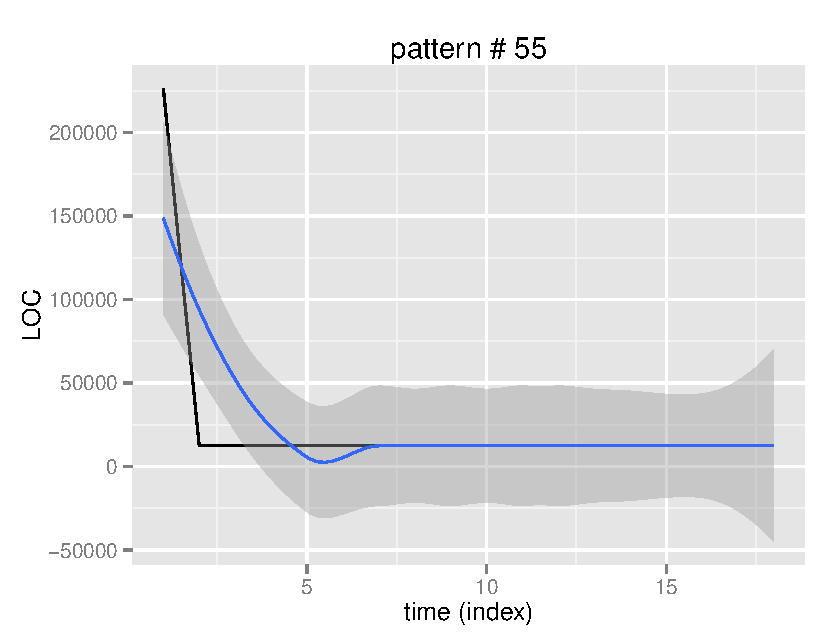
\includegraphics[width=128pt]{images/pattern_b_super.pdf}
\end{figure}

\noindent
Occurrences of type AB patterns are found anywhere in the evolution of dead
projects. This means that they may or may not be a candidate for representing a
warning sign. The difficulty is the fact that the AB patterns do not occur in a
consistent manner: in one project it may be an indicator for end of code
evolution, while in another project it does not.

\subsubsection{False-negatives}
When looking back at the projects selected for survival analysis in group G0
(section \ref{section:group_g0}), 4 out of 93 projects \textit{not} having a
type A pattern died. The patterns indicating the impending end of code
evolution were not detected as such. However, all 4 projects had occurrences of
type AB patterns.

Evaluation showed that the 42 AB patterns from the four projects in group
G0 all show a stagnation in LOC change. The difficulty is that the type AB
patterns also occur somewhere else in a dead project's evolution, which cannot
be identified uniformly as possible warning signs.

\subsubsection{False-positives}
Taking the projects in group G1 (section \ref{section:group_g1}), 79 out of 93
projects were still alive by April 2014. The alive projects already lived
longer since diagnosis than the dead projects in the same group. This means
that not all patterns of type A can be interpreted as a warning sign.

\paragraph{}
It can be a possibility to treat AB patterns also as possible warning signs,
because of the property that in \textit{some} projects the pattern occurs near,
and lasts until the end of code evolution. This, however, will yield more
false-positive results because a pattern occurring anywhere in a project's
evolution could hardly be an indicator of the end of that evolution.
On the other hand, treating the AB patterns explicitly \textit{not} as possible
warning signs -- as in this study -- will yield more false-negative results.

\section{Survival analysis}
\label{section:kp_survival}
The Kaplan-Meier estimation of the survival function of the projects as shown
in Figure \ref{figure:kp_survival} suggests that projects in group G1 -- the
projects having an occurrence of a type A pattern -- die earlier than the
projects in group G0 -- the projects without an occurrence of a type A pattern.

\paragraph{}
The four dead projects of G0 die in their first 14 months (see section
\ref{section:group_g0}). This causes both strata in the curve to diverge a
little and gives the impression that the projects of group G1 have a higher
chance of survival than those of group G0, at least for the first 3 years.

Two of the dead projects in G0 are small ($<$ 5,000 LOC), the other two
quite large ($>$ 150,000 LOC). However, the larger two have had their LOC value
since the very first data point. This suggests that these projects were
developed outside of source control and at one time everything was committed at
once. The total number of commits in the history of the projects confirms this:
both projects have less than 30 commits in their entire 2 year history.

The smaller two projects have had 40 and 60 commits in respectively 3 and 4
years time. The four projects could therefore as well be outliers that cause a
slight distortion in the curve.


\section{Threats to validity}
The following aspects were found which may lead to threats to the validity of
the results.

\begin{description}
	\item[Construct validity] \hfill
	
	\begin{description}
		\item[\rm{Missing historical data}] -- In the analysis of project's
			evolution data, only the data provided by the OhlohAnalytics tool
			\cite{ohlohanalytics, bruntink2013} was used.
			The data before the first data point in the set is not taken into account. It
			is possible that certain evolutionary events happened before the first point.
			These events were not detected as they lay beyond reach of this study.

		\item[\rm{Missing most recent data}] -- The data provided for the study has
			data points until June 2013. Therefore, not the most recent data of the
			projects is used.

		\item[\rm{LOC as activity indicator}] -- The use of LOC (defined as
			lines of code + comments + blanks) as a measure of project activity could be
			false. The LOC will not change between two months whenever the amount of code
			deleted is equal to the amount added. In that case, the churn would be twice
			the LOC added/deleted, but the LOC will stay the same.

			When patterns are detected that show a stagnation in LOC, the suggestion
			would be that the project's activity is decreasing. However, it might also
			be the case that by coincidence it seems activity is decreasing, but in
			reality lots of activity has been going on.

		\item[\rm{Data source}] -- Using only one data source (Ohloh) may
			influence the value of the metrics. Ohloh did the analysis of the project's
			source code repositories. Several studies have shown that the data provided
			by Ohloh needs a thorough examination and cleansing before it can be used
			\cite{bruntink2013, ohlohanalytics, bruntink2014}. The data was initially
			validated and cleansed to make it consistent, but no actual verification on
			the correctness of the data was conducted.
	\end{description}

	\item[Internal validity] \hfill

	\begin{description}
		\item[\rm{Selection bias}] -- The selection criteria for the data was to have
			at least 12 data points. It turned out, no project in the set was younger
			than 14 months. It might be that these younger projects show significance in
			the ability to detect evolutionary events, possibly refute or confirm
			findings.
	\end{description}

	\item[External validity] \hfill

	\begin{description}
		\item[\rm{Replication}] -- It seems hard to precisely replicate the study
			as there are a multitude of possible configurations to be made that may, in
			the end, influence the results drastically. Such as, the definition of
			similarity between sequences (what deviation is allowed, what is the
			difference of coincidence and a reoccurring sequence), and the definition of
			a pattern (how many occurrences, minimum, and maximum length).
			
			Furthermore, there is the interpretation of what a 'warning sign' should
			look like on a pattern level.
	\end{description}
\end{description}

\section{Future work}
A next step in the research on the use of wavelet analysis for detecting
warning signs in software evolution would be to use a larger data set. It would
be interesting to know if the findings of the type A patterns will be
consistent. The whole usable data set for this study contains 5,986 projects
(section \ref{method:data}).

\paragraph{}
The analysis could be done on other signals. In this study, only LOC was used,
but many other signals can be constructed. LOC evolution measures code activity
to a certain extent, but LOC churn could reflect code activity better. To use
LOC churn properly, the LOC modified fact is also needed.

Other useful metrics for finding warning signs could be team size, developer's
churn (the number of developers added and removed from the team), contributor's
code activity, bug reports, and defects per kLOC.

\begin{comment}
- Analyse results
- Conclude and interpret results
- Answer hypotheses and research questions
- Threats to validity
- Discussion
- Future work
 
This chapter contains the analysis and interpretation of the results. The
research questions are answered as best as possible given the results that were
obtained. The analysis also discussed parts of the questions that were left
unanswered.

An important topic is the validity of the results.
What methods of validation were used?
Could the results be generalized to other cases?
What threats to validity can be identified?

There is room here to discuss the results of related scientific literature here
as well.
How do the results obtained here relate to other work, and what consequences are
there?
Did your approach work better or worse?
Did you learn anything new compared to the already existing body of knowledge?
Finally, what could you say in hindsight on the research approach by followed?
What could have done better?
What lessons have been learned?
What could other researchers use from your experience?

A separate section should be devoted to ‘future work,’ i.e., possible extension
points of your work that you have identified. Other researchers (or yourself)
could use those as a starting point.

Refer to Chapters 3.7 and 4 in this example thesis at Paul’s
homepage\footnote{http://homepages.cwi.nl/~paulk/thesesMasterSoftwareEngineering/2006/ReneWiegers.pdf}.
\end{comment}
